% Options for packages loaded elsewhere
% Options for packages loaded elsewhere
\PassOptionsToPackage{unicode}{hyperref}
\PassOptionsToPackage{hyphens}{url}
\PassOptionsToPackage{dvipsnames,svgnames,x11names}{xcolor}
%
\documentclass[
  letterpaper,
  DIV=11,
  numbers=noendperiod]{scrartcl}
\usepackage{xcolor}
\usepackage{amsmath,amssymb}
\setcounter{secnumdepth}{-\maxdimen} % remove section numbering
\usepackage{iftex}
\ifPDFTeX
  \usepackage[T1]{fontenc}
  \usepackage[utf8]{inputenc}
  \usepackage{textcomp} % provide euro and other symbols
\else % if luatex or xetex
  \usepackage{unicode-math} % this also loads fontspec
  \defaultfontfeatures{Scale=MatchLowercase}
  \defaultfontfeatures[\rmfamily]{Ligatures=TeX,Scale=1}
\fi
\usepackage{lmodern}
\ifPDFTeX\else
  % xetex/luatex font selection
\fi
% Use upquote if available, for straight quotes in verbatim environments
\IfFileExists{upquote.sty}{\usepackage{upquote}}{}
\IfFileExists{microtype.sty}{% use microtype if available
  \usepackage[]{microtype}
  \UseMicrotypeSet[protrusion]{basicmath} % disable protrusion for tt fonts
}{}
\makeatletter
\@ifundefined{KOMAClassName}{% if non-KOMA class
  \IfFileExists{parskip.sty}{%
    \usepackage{parskip}
  }{% else
    \setlength{\parindent}{0pt}
    \setlength{\parskip}{6pt plus 2pt minus 1pt}}
}{% if KOMA class
  \KOMAoptions{parskip=half}}
\makeatother
% Make \paragraph and \subparagraph free-standing
\makeatletter
\ifx\paragraph\undefined\else
  \let\oldparagraph\paragraph
  \renewcommand{\paragraph}{
    \@ifstar
      \xxxParagraphStar
      \xxxParagraphNoStar
  }
  \newcommand{\xxxParagraphStar}[1]{\oldparagraph*{#1}\mbox{}}
  \newcommand{\xxxParagraphNoStar}[1]{\oldparagraph{#1}\mbox{}}
\fi
\ifx\subparagraph\undefined\else
  \let\oldsubparagraph\subparagraph
  \renewcommand{\subparagraph}{
    \@ifstar
      \xxxSubParagraphStar
      \xxxSubParagraphNoStar
  }
  \newcommand{\xxxSubParagraphStar}[1]{\oldsubparagraph*{#1}\mbox{}}
  \newcommand{\xxxSubParagraphNoStar}[1]{\oldsubparagraph{#1}\mbox{}}
\fi
\makeatother

\usepackage{color}
\usepackage{fancyvrb}
\newcommand{\VerbBar}{|}
\newcommand{\VERB}{\Verb[commandchars=\\\{\}]}
\DefineVerbatimEnvironment{Highlighting}{Verbatim}{commandchars=\\\{\}}
% Add ',fontsize=\small' for more characters per line
\usepackage{framed}
\definecolor{shadecolor}{RGB}{241,243,245}
\newenvironment{Shaded}{\begin{snugshade}}{\end{snugshade}}
\newcommand{\AlertTok}[1]{\textcolor[rgb]{0.68,0.00,0.00}{#1}}
\newcommand{\AnnotationTok}[1]{\textcolor[rgb]{0.37,0.37,0.37}{#1}}
\newcommand{\AttributeTok}[1]{\textcolor[rgb]{0.40,0.45,0.13}{#1}}
\newcommand{\BaseNTok}[1]{\textcolor[rgb]{0.68,0.00,0.00}{#1}}
\newcommand{\BuiltInTok}[1]{\textcolor[rgb]{0.00,0.23,0.31}{#1}}
\newcommand{\CharTok}[1]{\textcolor[rgb]{0.13,0.47,0.30}{#1}}
\newcommand{\CommentTok}[1]{\textcolor[rgb]{0.37,0.37,0.37}{#1}}
\newcommand{\CommentVarTok}[1]{\textcolor[rgb]{0.37,0.37,0.37}{\textit{#1}}}
\newcommand{\ConstantTok}[1]{\textcolor[rgb]{0.56,0.35,0.01}{#1}}
\newcommand{\ControlFlowTok}[1]{\textcolor[rgb]{0.00,0.23,0.31}{\textbf{#1}}}
\newcommand{\DataTypeTok}[1]{\textcolor[rgb]{0.68,0.00,0.00}{#1}}
\newcommand{\DecValTok}[1]{\textcolor[rgb]{0.68,0.00,0.00}{#1}}
\newcommand{\DocumentationTok}[1]{\textcolor[rgb]{0.37,0.37,0.37}{\textit{#1}}}
\newcommand{\ErrorTok}[1]{\textcolor[rgb]{0.68,0.00,0.00}{#1}}
\newcommand{\ExtensionTok}[1]{\textcolor[rgb]{0.00,0.23,0.31}{#1}}
\newcommand{\FloatTok}[1]{\textcolor[rgb]{0.68,0.00,0.00}{#1}}
\newcommand{\FunctionTok}[1]{\textcolor[rgb]{0.28,0.35,0.67}{#1}}
\newcommand{\ImportTok}[1]{\textcolor[rgb]{0.00,0.46,0.62}{#1}}
\newcommand{\InformationTok}[1]{\textcolor[rgb]{0.37,0.37,0.37}{#1}}
\newcommand{\KeywordTok}[1]{\textcolor[rgb]{0.00,0.23,0.31}{\textbf{#1}}}
\newcommand{\NormalTok}[1]{\textcolor[rgb]{0.00,0.23,0.31}{#1}}
\newcommand{\OperatorTok}[1]{\textcolor[rgb]{0.37,0.37,0.37}{#1}}
\newcommand{\OtherTok}[1]{\textcolor[rgb]{0.00,0.23,0.31}{#1}}
\newcommand{\PreprocessorTok}[1]{\textcolor[rgb]{0.68,0.00,0.00}{#1}}
\newcommand{\RegionMarkerTok}[1]{\textcolor[rgb]{0.00,0.23,0.31}{#1}}
\newcommand{\SpecialCharTok}[1]{\textcolor[rgb]{0.37,0.37,0.37}{#1}}
\newcommand{\SpecialStringTok}[1]{\textcolor[rgb]{0.13,0.47,0.30}{#1}}
\newcommand{\StringTok}[1]{\textcolor[rgb]{0.13,0.47,0.30}{#1}}
\newcommand{\VariableTok}[1]{\textcolor[rgb]{0.07,0.07,0.07}{#1}}
\newcommand{\VerbatimStringTok}[1]{\textcolor[rgb]{0.13,0.47,0.30}{#1}}
\newcommand{\WarningTok}[1]{\textcolor[rgb]{0.37,0.37,0.37}{\textit{#1}}}

\usepackage{longtable,booktabs,array}
\usepackage{calc} % for calculating minipage widths
% Correct order of tables after \paragraph or \subparagraph
\usepackage{etoolbox}
\makeatletter
\patchcmd\longtable{\par}{\if@noskipsec\mbox{}\fi\par}{}{}
\makeatother
% Allow footnotes in longtable head/foot
\IfFileExists{footnotehyper.sty}{\usepackage{footnotehyper}}{\usepackage{footnote}}
\makesavenoteenv{longtable}
\usepackage{graphicx}
\makeatletter
\newsavebox\pandoc@box
\newcommand*\pandocbounded[1]{% scales image to fit in text height/width
  \sbox\pandoc@box{#1}%
  \Gscale@div\@tempa{\textheight}{\dimexpr\ht\pandoc@box+\dp\pandoc@box\relax}%
  \Gscale@div\@tempb{\linewidth}{\wd\pandoc@box}%
  \ifdim\@tempb\p@<\@tempa\p@\let\@tempa\@tempb\fi% select the smaller of both
  \ifdim\@tempa\p@<\p@\scalebox{\@tempa}{\usebox\pandoc@box}%
  \else\usebox{\pandoc@box}%
  \fi%
}
% Set default figure placement to htbp
\def\fps@figure{htbp}
\makeatother





\setlength{\emergencystretch}{3em} % prevent overfull lines

\providecommand{\tightlist}{%
  \setlength{\itemsep}{0pt}\setlength{\parskip}{0pt}}



 


\KOMAoption{captions}{tableheading}
\makeatletter
\@ifpackageloaded{tcolorbox}{}{\usepackage[skins,breakable]{tcolorbox}}
\@ifpackageloaded{fontawesome5}{}{\usepackage{fontawesome5}}
\definecolor{quarto-callout-color}{HTML}{909090}
\definecolor{quarto-callout-note-color}{HTML}{0758E5}
\definecolor{quarto-callout-important-color}{HTML}{CC1914}
\definecolor{quarto-callout-warning-color}{HTML}{EB9113}
\definecolor{quarto-callout-tip-color}{HTML}{00A047}
\definecolor{quarto-callout-caution-color}{HTML}{FC5300}
\definecolor{quarto-callout-color-frame}{HTML}{acacac}
\definecolor{quarto-callout-note-color-frame}{HTML}{4582ec}
\definecolor{quarto-callout-important-color-frame}{HTML}{d9534f}
\definecolor{quarto-callout-warning-color-frame}{HTML}{f0ad4e}
\definecolor{quarto-callout-tip-color-frame}{HTML}{02b875}
\definecolor{quarto-callout-caution-color-frame}{HTML}{fd7e14}
\makeatother
\makeatletter
\@ifpackageloaded{caption}{}{\usepackage{caption}}
\AtBeginDocument{%
\ifdefined\contentsname
  \renewcommand*\contentsname{Table of contents}
\else
  \newcommand\contentsname{Table of contents}
\fi
\ifdefined\listfigurename
  \renewcommand*\listfigurename{List of Figures}
\else
  \newcommand\listfigurename{List of Figures}
\fi
\ifdefined\listtablename
  \renewcommand*\listtablename{List of Tables}
\else
  \newcommand\listtablename{List of Tables}
\fi
\ifdefined\figurename
  \renewcommand*\figurename{Figure}
\else
  \newcommand\figurename{Figure}
\fi
\ifdefined\tablename
  \renewcommand*\tablename{Table}
\else
  \newcommand\tablename{Table}
\fi
}
\@ifpackageloaded{float}{}{\usepackage{float}}
\floatstyle{ruled}
\@ifundefined{c@chapter}{\newfloat{codelisting}{h}{lop}}{\newfloat{codelisting}{h}{lop}[chapter]}
\floatname{codelisting}{Listing}
\newcommand*\listoflistings{\listof{codelisting}{List of Listings}}
\makeatother
\makeatletter
\makeatother
\makeatletter
\@ifpackageloaded{caption}{}{\usepackage{caption}}
\@ifpackageloaded{subcaption}{}{\usepackage{subcaption}}
\makeatother
\usepackage{bookmark}
\IfFileExists{xurl.sty}{\usepackage{xurl}}{} % add URL line breaks if available
\urlstyle{same}
\hypersetup{
  pdftitle={Chapter 8 - Classification and Generalized regression: Exercise solutions},
  pdfauthor={Mattias Villani},
  colorlinks=true,
  linkcolor={blue},
  filecolor={Maroon},
  citecolor={Blue},
  urlcolor={Blue},
  pdfcreator={LaTeX via pandoc}}


\title{Chapter 8 - Classification and Generalized regression: Exercise
solutions}
\author{Mattias Villani}
\date{}
\begin{document}
\maketitle


Click on the arrow to see a solution.

\subsubsection{Exercise 8.1}\label{exercise-8.1}

The dataset \texttt{runningtime.csv} available at
\url{https://github.com/mattiasvillani/BayesianLearningBook/raw/main/data/runningtime.csv}
contains measurements on the running time (\texttt{time}) for a computer
code on \(n=100\) computers with different hardware specifications and
operating systems. The performance score summarized by a normalized
performance score (\texttt{performance}), where a higher score means
better performance. The operating system is either Windows
(\texttt{os=1}) or Linux (\texttt{os=0}).

Consider the following exponential regression model \begin{equation*}
   y_i \vert \mathbf{x}_i,\boldsymbol{\beta} \sim \mathrm{Expon}\left(\frac{1}{\exp\left(\mathbf{x}_i^\top \boldsymbol{\beta}\right)}\right)
  \end{equation*} for \(i=1,\ldots,n\), where \(y_i\) is the response
variable, \(\mathbf{x}\) is a vector with three elements, the first
element is \(1\) for the intercept, the second element is the
performance measure for the \(i\)th computer and the final element if
the operating system for the computer. Note the
\(\mathbb{E}(y_i \vert \mathbf{x}_i) = \exp\left(\mathbf{x}_i^\top \boldsymbol{\beta}\right)\)
for this model. Let the prior be
\(\beta\sim N(\boldsymbol{0},\lambda^{-1}\boldsymbol{I}_3)\), where
\(\lambda=1\) and \(\boldsymbol{I}_3\) is the \(3 \times 3\) identity
matrix.

\begin{enumerate}[(a)]
    \item   \input{exercises/classification/expon_reg_approx_a.tex}
    \item   \input{exercises/classification/expon_reg_approx_b.tex}
\end{enumerate}

Loading the data and mvtnorm package

\begin{Shaded}
\begin{Highlighting}[]
\FunctionTok{library}\NormalTok{(mvtnorm)}
\NormalTok{data }\OtherTok{=} \FunctionTok{read.csv}\NormalTok{(}\StringTok{"https://raw.githubusercontent.com/mattiasvillani/BayesianLearningBook/main/data/runningtime.csv"}\NormalTok{)}
\NormalTok{y }\OtherTok{=}\NormalTok{ data}\SpecialCharTok{$}\NormalTok{time}
\NormalTok{X }\OtherTok{=} \FunctionTok{cbind}\NormalTok{(}\DecValTok{1}\NormalTok{, data}\SpecialCharTok{$}\NormalTok{performance, data}\SpecialCharTok{$}\NormalTok{os)}
\FunctionTok{hist}\NormalTok{(y, }\DecValTok{30}\NormalTok{, }\AttributeTok{freq =} \ConstantTok{FALSE}\NormalTok{, }\AttributeTok{main =} \StringTok{"The running time data"}\NormalTok{, }\AttributeTok{xlab =} \StringTok{"running time"}\NormalTok{)}
\end{Highlighting}
\end{Shaded}

\pandocbounded{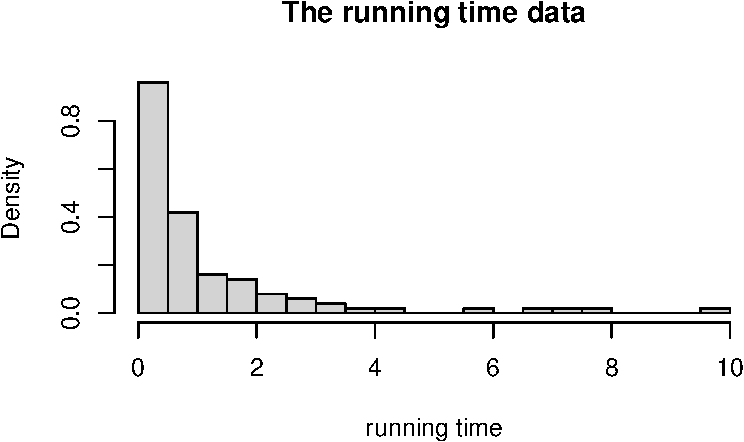
\includegraphics[keepaspectratio]{ch8solutions_files/figure-pdf/unnamed-chunk-2-1.pdf}}

\textbf{a)} Do a normal approximation of the posterior distribution
\(p(\boldsymbol{\beta} | \mathbf{y},\mathbf{X})\) based on numerical
optimization. Simulate \numprint{10000} samples from this approximation
and make histograms to approximate the marginal posterior for each
parameter in \(\beta\).

\begin{tcolorbox}[enhanced jigsaw, rightrule=.15mm, colframe=quarto-callout-note-color-frame, arc=.35mm, leftrule=.75mm, bottomtitle=1mm, opacityback=0, coltitle=black, colbacktitle=quarto-callout-note-color!10!white, left=2mm, toptitle=1mm, breakable, toprule=.15mm, titlerule=0mm, title={Solution}, bottomrule=.15mm, colback=white, opacitybacktitle=0.6]

We will use optim to get the posterior mode and posterior observed
information matrix for the normal approximation. The log posterior
function is

\begin{Shaded}
\begin{Highlighting}[]
\NormalTok{logPostExpon }\OtherTok{\textless{}{-}} \ControlFlowTok{function}\NormalTok{(betaVect, y, X, tau)\{}
\NormalTok{  p }\OtherTok{\textless{}{-}} \FunctionTok{length}\NormalTok{(betaVect)}
\NormalTok{  linPred }\OtherTok{\textless{}{-}}\NormalTok{ X}\SpecialCharTok{\%*\%}\NormalTok{betaVect}
\NormalTok{  logLik }\OtherTok{\textless{}{-}} \FunctionTok{sum}\NormalTok{(}\FunctionTok{dexp}\NormalTok{(y, }\AttributeTok{rate =} \DecValTok{1}\SpecialCharTok{/}\FunctionTok{exp}\NormalTok{(linPred), }\AttributeTok{log =} \ConstantTok{TRUE}\NormalTok{) )}
\NormalTok{  logPrior }\OtherTok{\textless{}{-}} \FunctionTok{dmvnorm}\NormalTok{(betaVect, }\FunctionTok{rep}\NormalTok{(}\DecValTok{0}\NormalTok{, p), tau}\SpecialCharTok{\^{}}\DecValTok{2}\SpecialCharTok{*}\FunctionTok{diag}\NormalTok{(p), }\AttributeTok{log=}\ConstantTok{TRUE}\NormalTok{)}
  \FunctionTok{return}\NormalTok{(logLik }\SpecialCharTok{+}\NormalTok{ logPrior)}
\NormalTok{\}}
\end{Highlighting}
\end{Shaded}

We use optim to find the posterior mode and posterior information
matrix:

\begin{Shaded}
\begin{Highlighting}[]
\NormalTok{p }\OtherTok{=} \FunctionTok{dim}\NormalTok{(X)[}\DecValTok{2}\NormalTok{]}
\NormalTok{tau }\OtherTok{=} \DecValTok{10}
\NormalTok{initVal }\OtherTok{\textless{}{-}} \FunctionTok{as.vector}\NormalTok{(}\FunctionTok{rep}\NormalTok{(}\DecValTok{0}\NormalTok{,p))}
\NormalTok{OptimResults}\OtherTok{\textless{}{-}}\FunctionTok{optim}\NormalTok{(initVal, logPostExpon,}\AttributeTok{gr=}\ConstantTok{NULL}\NormalTok{, y, X, tau,}
  \AttributeTok{method=}\FunctionTok{c}\NormalTok{(}\StringTok{"BFGS"}\NormalTok{), }\AttributeTok{control=}\FunctionTok{list}\NormalTok{(}\AttributeTok{fnscale=}\SpecialCharTok{{-}}\DecValTok{1}\NormalTok{), }\AttributeTok{hessian=}\ConstantTok{TRUE}\NormalTok{)}
\NormalTok{postMode }\OtherTok{=}\NormalTok{ OptimResults}\SpecialCharTok{$}\NormalTok{par}
\NormalTok{postCov }\OtherTok{=} \SpecialCharTok{{-}}\FunctionTok{solve}\NormalTok{(OptimResults}\SpecialCharTok{$}\NormalTok{hessian) }\CommentTok{\# inv(J) {-} Approx posterior covariance matrix}
\NormalTok{postStd }\OtherTok{=} \FunctionTok{sqrt}\NormalTok{(}\FunctionTok{diag}\NormalTok{(postCov))}
\end{Highlighting}
\end{Shaded}

Simulating from the normal approximation and plotting histograms of the
marginal posteriors:

\begin{Shaded}
\begin{Highlighting}[]
\NormalTok{nSim }\OtherTok{=} \DecValTok{10000}
\FunctionTok{library}\NormalTok{(mvtnorm)}
\NormalTok{betaDraws }\OtherTok{=} \FunctionTok{rmvnorm}\NormalTok{(nSim, postMode, postCov)}
\FunctionTok{par}\NormalTok{(}\AttributeTok{mfrow =} \FunctionTok{c}\NormalTok{(}\DecValTok{1}\NormalTok{,p))}
\NormalTok{varNames }\OtherTok{=} \FunctionTok{c}\NormalTok{(}\StringTok{"intercept"}\NormalTok{, }\StringTok{"performance"}\NormalTok{, }\StringTok{"os"}\NormalTok{)}
\ControlFlowTok{for}\NormalTok{ (j }\ControlFlowTok{in} \DecValTok{1}\SpecialCharTok{:}\NormalTok{p)\{}
\FunctionTok{hist}\NormalTok{(betaDraws[,j], }\DecValTok{30}\NormalTok{, }\AttributeTok{freq =} \ConstantTok{FALSE}\NormalTok{, }\AttributeTok{main =}\NormalTok{ varNames[j], }
     \AttributeTok{xlab =} \StringTok{""}\NormalTok{, }\AttributeTok{col =} \StringTok{"cornflowerblue"}\NormalTok{)}
\NormalTok{\}}
\end{Highlighting}
\end{Shaded}

\pandocbounded{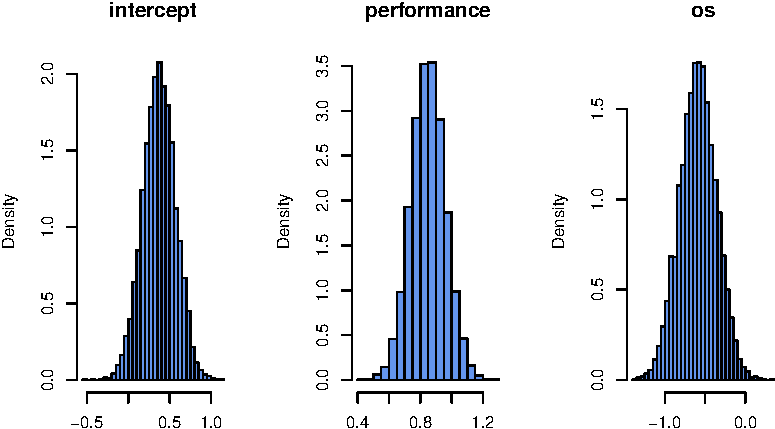
\includegraphics[keepaspectratio]{ch8solutions_files/figure-pdf/unnamed-chunk-5-1.pdf}}

\end{tcolorbox}

\textbf{b)} Use the normal approximation from a) and simulation to
approximate the predictive distribution of the running time for a new
Windows computer with performance measure equal to \(1.3\).

\begin{tcolorbox}[enhanced jigsaw, rightrule=.15mm, colframe=quarto-callout-note-color-frame, arc=.35mm, leftrule=.75mm, bottomtitle=1mm, opacityback=0, coltitle=black, colbacktitle=quarto-callout-note-color!10!white, left=2mm, toptitle=1mm, breakable, toprule=.15mm, titlerule=0mm, title={Solution}, bottomrule=.15mm, colback=white, opacitybacktitle=0.6]

\begin{Shaded}
\begin{Highlighting}[]
\NormalTok{xPred }\OtherTok{=} \FunctionTok{c}\NormalTok{(}\DecValTok{1}\NormalTok{, }\FloatTok{1.3}\NormalTok{, }\DecValTok{1}\NormalTok{)}
\NormalTok{yPredDraws }\OtherTok{=} \FunctionTok{rep}\NormalTok{(}\DecValTok{0}\NormalTok{, nSim)}
\ControlFlowTok{for}\NormalTok{ (i }\ControlFlowTok{in} \DecValTok{1}\SpecialCharTok{:}\NormalTok{nSim)\{}
\NormalTok{  yPredDraws[i] }\OtherTok{=} \FunctionTok{rexp}\NormalTok{(}\DecValTok{1}\NormalTok{, }\FunctionTok{exp}\NormalTok{(xPred }\SpecialCharTok{\%*\%}\NormalTok{ betaDraws[i,]))}
\NormalTok{\}}
\FunctionTok{hist}\NormalTok{(yPredDraws, }\DecValTok{30}\NormalTok{, }\AttributeTok{freq =} \ConstantTok{FALSE}\NormalTok{, }\AttributeTok{main =} \StringTok{"Predictive density"}\NormalTok{, }
     \AttributeTok{xlab =} \StringTok{"yPred"}\NormalTok{, }\AttributeTok{col =} \StringTok{"cornsilk"}\NormalTok{)}
\end{Highlighting}
\end{Shaded}

\pandocbounded{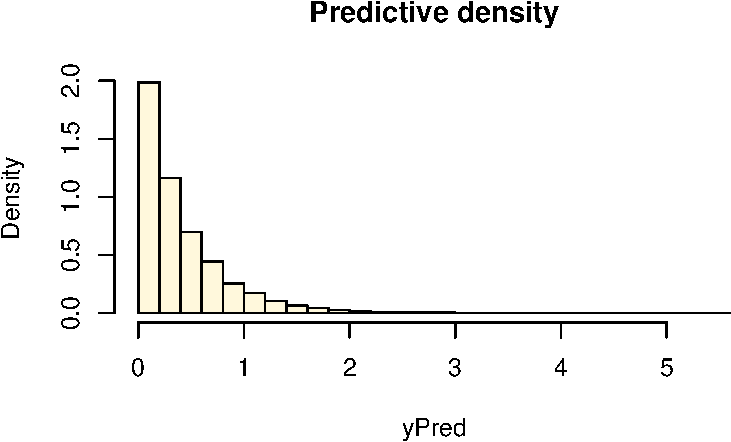
\includegraphics[keepaspectratio]{ch8solutions_files/figure-pdf/unnamed-chunk-6-1.pdf}}

\end{tcolorbox}




\end{document}
